\begin{figure}[h]
    \centering
    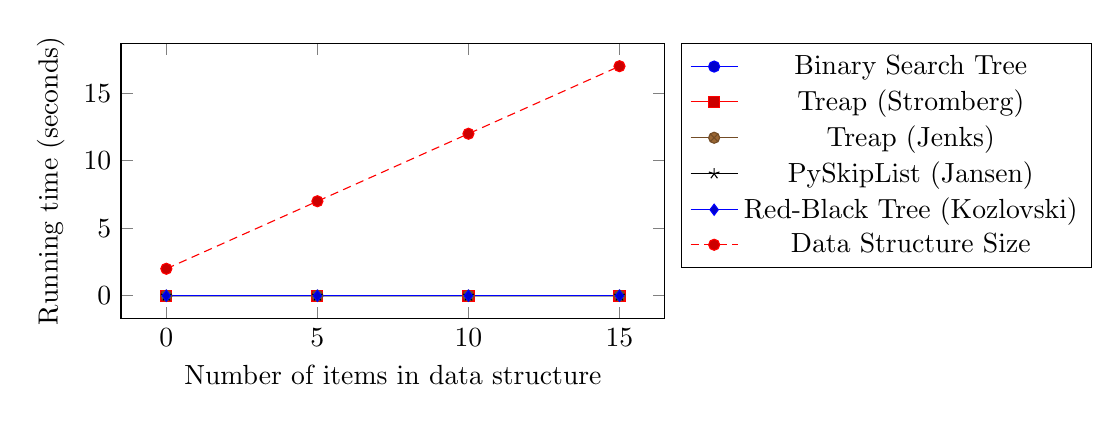
\begin{tikzpicture}
        \begin{axis}[
            xlabel={Number of items in data structure},
            ylabel={Running time (seconds)},
            title={},
            width=0.7\textwidth,
            height=2in,
            legend pos=outer north east
        ]
		\addplot coordinates {
			(0, 3.81488759885453e-06)
			(5, 2.8109698096822854e-06)
			(10, 2.6101862518478425e-06)
			(15, 2.9113615885995115e-06)
		};
		\addplot coordinates {
			(0, 7.328599860957387e-06)
			(5, 7.629775197709075e-06)
			(10, 7.2282080820401705e-06)
			(15, 7.3285998609573695e-06)
		};
		\addplot coordinates {
			(0, 8.533301207964083e-06)
			(5, 7.930950534460745e-06)
			(10, 6.826640966371266e-06)
			(15, 7.830558755543546e-06)
		};
		\addplot coordinates {
			(0, 1.214740524898415e-05)
			(5, 1.3954457269494238e-05)
			(10, 1.234818880681862e-05)
			(15, 1.2850147701404723e-05)
		};
		\addplot coordinates {
			(0, 8.934868323632987e-06)
			(5, 6.826640966371194e-06)
			(10, 6.826640966371266e-06)
			(15, 6.927032745288429e-06)
		};
		\addplot coordinates {
			(0, 2)
			(5, 7)
			(10, 12)
			(15, 17)
		};
        \legend{Binary Search Tree, Treap (Stromberg), Treap (Jenks), PySkipList (Jansen), Red-Black Tree (Kozlovski), Data Structure Size}
        \end{axis}
    \end{tikzpicture}
    \caption{Average of 3 operations, benchmarked every 5, starting at 0.}
\end{figure}